\documentclass{article}
\usepackage[margin=1in]{geometry}
\usepackage{enumerate}
\usepackage{ textcomp }
\usepackage[pdftex]{graphicx}
\usepackage{float}

\title{3D EBSD Boundary Characterization\\ {\normalsize Aluminum Sample from Valerie Randle}}	
	
\author{David Golay, Andrew Loeb, Ayyappa Vemulkar\\
Professor Lori Bassman
}		
\date{May 27, 2012}				
\begin{document}

\maketitle

This document explains the methods used to characterize grain boundaries in the 3D EBSD data set that we collected on the aluminum sample from Valerie Randle. The attachments contain the results of this analysis and are indexed at the end of the document.


\section{Segmentation}
The 3D EBSD data were taken using a \textit{Zeiss Auriga Cross Beam} microscope, with 32 slices of 0.5 micron thickness. Each slice is approximately 60$\times$21 microns with 0.5 micron spacing between points. The data were cleaned (one pass of noise reduction at default levels), cropped and segmented using \textit{Oxford HKL 3D Viewer} software. In-house {\sc matlab} code was used for all further analysis. Boundaries between grains were isolated and can be seen in Figure \ref{surfaces}.

\begin{figure}[h]
  \centering
    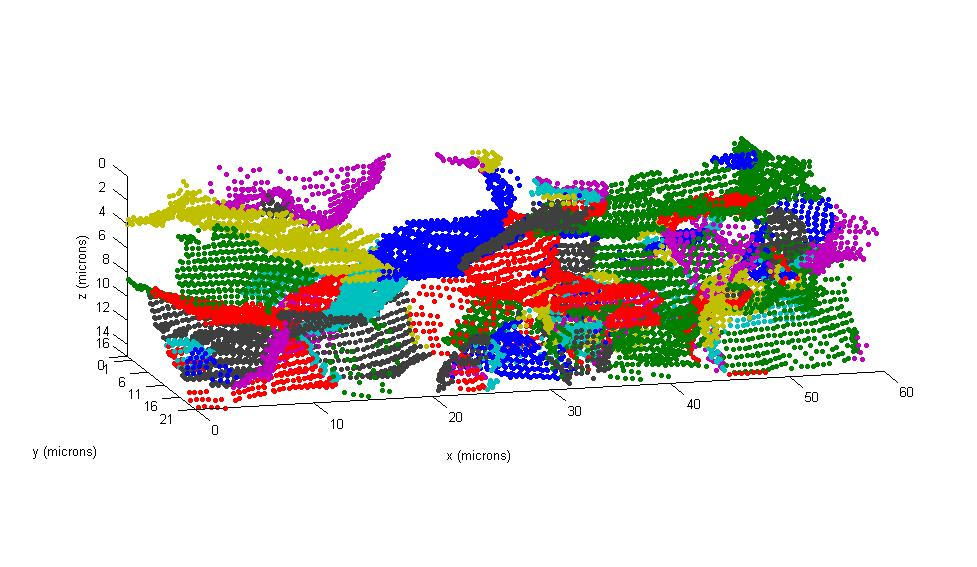
\includegraphics[width=0.8\textwidth]{surfacesVal.jpg}
  \caption{Plot of all grain boundary surfaces}
  \label{surfaces}
\end{figure}

The segmentation produced 70 clusters. Fifty-four of the clusters are clearly distinct grains (standard deviations of orientations within each is less than 1.4 degrees). However, some clusters seem undersegmented. Figure \ref{underseg} shows a cluster with relative orientations depicted in color. This cluster (number 27) contains two, and possibly three, distinct regions. However, each of the boundaries between these clusters and adjacent grains seems to be confined to single regions. That is, surfaces do not span these undersegmented regions. Thus, although some boundaries are missing, analysis on the surfaces that were generated is still valid. The full list of undersegmented clusters is below, and caution should still be taken when working with their boundaries. $$\mbox{Clusters }[0-2-3-6-7-12-14-15-18-20-21-23-24-25-27-57]$$

\begin{figure}[h]
  \centering
    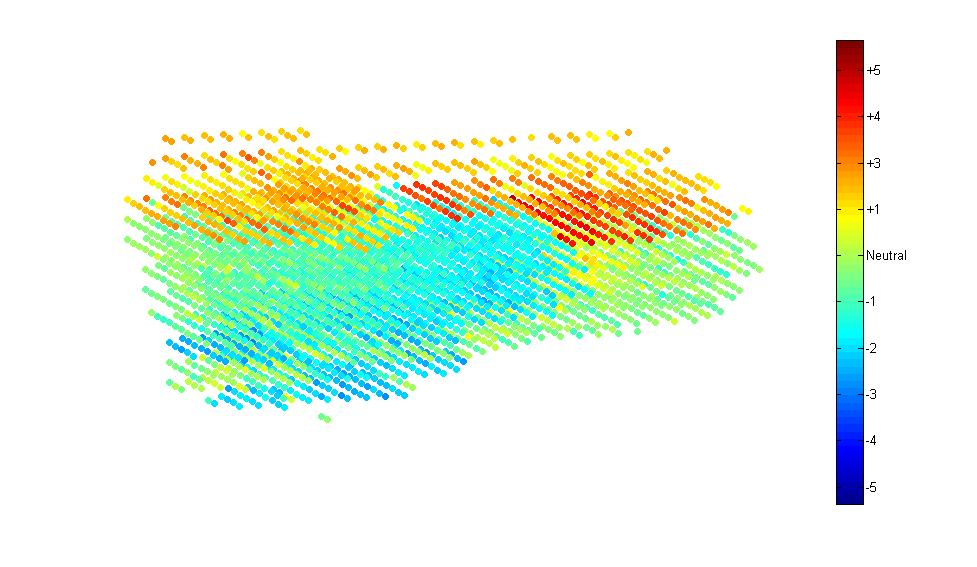
\includegraphics[width=.8\textwidth]{underseg.jpg}
  \caption{Relative orientations within cluster 27}
  \label{underseg}
\end{figure}

\section{Misorientation Between Grains}
Two methods were used to determine misorientation between grains: the difference between average grain orientations (using all points in the volumes), and average pointwise misorientation (using all adjacent points on the grain surfaces). These data are stored in \texttt{misAgg} and \texttt{misP2P}, respectively. These are upper-triangular arrays containing the misorientations between the $i^{th}$ and $j^{th}$ grains. Figure \ref{avp} shows a greyscale mapping of these two arrays concatenated together. The approximate diagonal symmetry shows the similarity of the two methods. 

\begin{figure}[h]
  \centering
    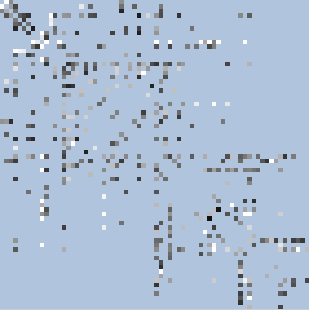
\includegraphics[width=0.32\textwidth]{aggVsP2P.PNG}
  \caption{Mapping of intergrain misorientations. The lower triangle represents comparison of average grain orientations and the upper triangle represents pointwise misorientations across boundaries. Grain pairs that do not share a boundary are blue.}
  \label{avp}
\end{figure}


\section{Surface Normals}
The local normals for each boundary were found and the average Cartesian components of these are stored in \texttt{surfNormsX}, \texttt{surfNormsY}, and \texttt{surfNormsZ}. These vectors are oriented with respect to the axes of the data set (with the Z-axis oriented down, as in Figure \ref{surfaces}). An example surface (between grains 9 and 10) is shown in Figure \ref{normal}.

\begin{figure}[h]
  \centering
    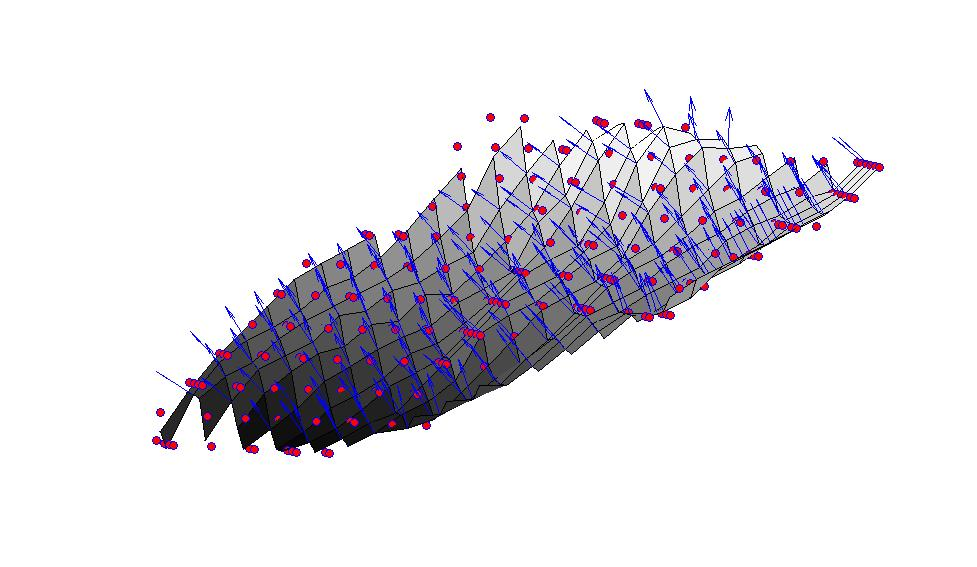
\includegraphics[width=0.9\textwidth]{normal.jpg}
  \caption{Plot of the boundary between grains 9 and 10 with local surface normals shown.}
  \label{normal}
\end{figure}

\pagebreak 

\section{Attachments}
All attached files are listed below.

\begin{center}
\begin{tabular}{l l}
\texttt{VR aluminum 3D cropped and cleaned.ctf}&Raw EBSD data containing Cartesian coordinates,\\
& Euler angle, and grain number of every point\\
\texttt{VR aluminum 3D cropped and cleaned2.txt}&Tab delineated EBSD data for {\sc matlab} import\\
\texttt{Boundaries.txt}&Coordinates of every point on a grain boundary\\
& with local misorientation between grains\\
\texttt{grainOrien.txt}&Average quaternion orientation of each grain\\
\texttt{misAgg.txt}&Misorientations between grains calculated on grain average\\
\texttt{misP2P.txt}&Misorientations calculated pointwise across boundaries\\
\texttt{surfNormsX.txt}&X components of normal vectors for each boundary surface\\
\texttt{surfNormsY.txt}&Y components of normal vectors for each boundary surface\\
\texttt{surfNormsZ.txt}&Z components of normal vectors for each boundary surface\\
\end{tabular}
\end{center}




\end{document}